\subsection{Основное уравнение динамики вращательного движения твердого тела с закрепленной осью вращения. Момент импульса тела. Момент инерции}

\begin{definition}
    Основное уравнение динамики вращательного движения твёрдого тела с закрепленной осью вращения.

    $$I\cdot\vec\varepsilon=\sum_i\vec M_i$$

    Произведение момента инерции твёрдого тела относительно оси вращения на его угловое ускорение равно сумме моментов внешних сил относительно той же оси.
\end{definition}

\begin{definition}
    Момент импульса твёрдого тела.

    $$\vec L=I\cdot\vec\omega$$

    Момент импульса абсолютно твёрдого тела относительно оси вращения равен произведению его момента инерции относительно той же оси на угловую скорость.
\end{definition}

\begin{definition}
    Момент инерции твёрдого тела 

    Момент инерции зависит от массы тела и от того, как распределена масса относительно оси вращения.

    По одной и той же массе тела момент инерции может быть разным.

    $$I=\sum_iI_i=\sum_i\Delta m_i\ r_i^2$$

    Для непрерывного распределения массы момент инерции — предел, к которому стремится сумма:

    $$I=\int r^2dm$$
\end{definition}

\begin{figure}[h]
    \centering
    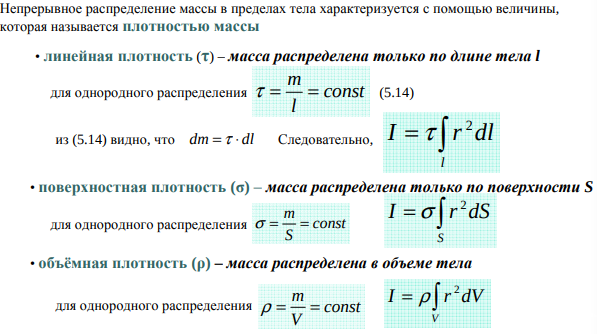
\includegraphics[width=0.7\linewidth]{imgs/q9i1.png}
\end{figure}